\chapter{Introduction}
\label{cha:intro}
Cloud computing is a model for enabling ubiquitous, convenient, on-demand network access to a shared pool of configurable computing resources (e.g., networks, servers, storage, applications, and services) that can be rapidly provisioned and released with minimal management effort or service provider interaction. This cloud model is composed of five essential characteristics, three service models, and four deployment models \cite{NIST}. The five essential characteristics are: on-demand self-service, broad network access, resource pooling, rapid elasticity, measured service. The four deployment models are: Public, Private, Hybrid and Community.

The 3 Cloud service models are: Software as
a Service (SaaS), Platform as a Service (PaaS), and
Infrastructure as a Service (IaaS). 
\Cref{fig:ArchitectureOfCloud} by Hitachi illustrates the architecture and general components of the Cloud.

\begin{figure}[ht]
  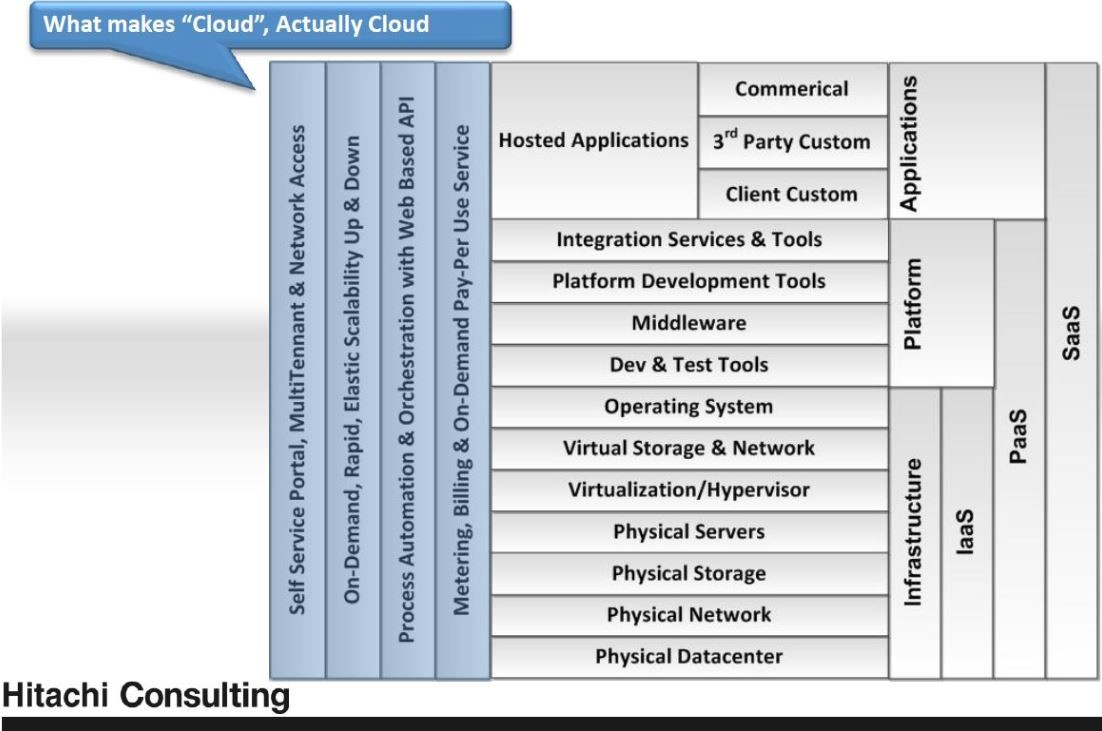
\includegraphics[width=\textwidth]{Figures/intro/Hitachi_3Layers.jpg}
  \caption{Architecture of the Cloud}
  \label{fig:ArchitectureOfCloud}
\end{figure}

Within the infrastructure layer, hypervisor software \cite{xen}
enables flexible provisioning of Virtual Machine, Storage and Network services.
On top of Infrastructure layer, additional Middleware, Tools or Integration Services can be provided as PaaS. Apps can also be hosted on IaaS and PaaS, those software available to customer at pay as you go model are SaaS.
The top layer focuses on application services by making
use of services provided by the lower layers. PaaS/SaaS
services can be developed and provided by third party
service providers who are different from the IaaS providers.
Some examples of SaaS providers are: Salesforce.com, Microsoft Office 365,
Oracle CRM On Demand, Goggle Apps.
Some examples of PaaS providers are: Google App Engine,
Force.com, Heroku. 
Some examples of IaaS providers are: Amazon Web Service \cite{aws}, Google Compute Engine \cite{google_cloud}, Microsoft Azure, Rackspace \cite{Rackspace}, Alibaba Cloud \cite{Alibaba}, IBM Softlayer \cite{IBMSoftLayer}, FlexiScale \cite{FlexiScale}, DataCentred \cite{DataCentred}.

In a cloud computing model, users access services according
to their requirements without the need to know where the
services are hosted or how they are delivered. 
Cloud computing embraces an elastic paradigm in which applications establish on-demand
interactions with services to satisfy required Quality of Service (QoS) including cost,
response time and throughput.

As Cloud continues to revolutionize applications in academia, industry, government, and many other fields, the transition to this efficient and flexible platform presents serious challenges at both theoretical and practical levels \cite{CloudComputingMethodologySystemsApplications}.
Just as large ISPs use multiple network providers so that failure by a single company
will not take them off the air,
the only plausible solution to very high availability
is multiple cloud computing providers \cite{Armbrust:2010:VCC:1721654.1721672}.
However, selecting and composing the right services
meeting application requirements is a challenging problem.
Consider an example of a medium scale enterprise that would like to move its
enterprise applications to Cloud.
There are multiple providers that offer infrastructure services in various configurations.
Examples include, Amazon , Microsoft Azure, Google, Alibaba among many others.
With varied options, enterprises are facing a complex task when trying to select a single service or compose a combination of services.
Here we are concerned with how to simplify the selection and comparison of a set of
infrastructure service offerings for hosting the enterprise applications and
corresponding datasets, while meeting multiple criteria, such as specific configuration
and cost, emanating from the enterprise’s QoS needs.
This is a challenging problem for the enterprise and needs to be addressed.

\section{Challenges in Cloud Selection and Comparison}
\label{sec:research_problem}
Since the prediction of Cloud bearing a trillion dollar market \cite{Market-OrientedCloudComputing}, it's exploding growth has fulfilled the prophecy.
With the proliferation of a range of Cloud services over the
Internet, efficient and accurate service discovery and selection
based on user-specific requirements has become a significant challenge for decision makers \cite{SMICloud}. This thesis will focus on the following problems.

\subsection{Confusing and Ambiguous Terminology}
\label{subsec:Non-standardizedAmbiguousTerminology}
Cloud providers use non-standardized naming terminologies for self branding their uniqueness. 
For example, the Compute services 
can be called Elastic Compute Cloud (EC2) Unit by AWS, Compute Engine by Google, 
Elastic Compute Service (ECS) by Alibaba, or just Virtual Machines (VMs), Instances, Servers or Units by others. NIST definition describes such service as the provision of processing computing resources.

Ambiguous terminologies are often used to describe similar configurations,
for instance different units of measurements are used for similar metrics.
One example is the CPU clock speed. Amazon refers to it as “ECUs”\cite{AmazonEC2}:
“\textit{One EC2 Compute Unit provides the equivalent COMPUTE capacity of a 1.0-1.2 GHz 2007 Opteron or 2007 Xeon processor. This is also the equivalent to an early-2006 1.7 GHz Xeon processor referenced in our original documentation}”.
In 2007, AMD and Intel released both dual-core and quad-core models of the Opteron and Xeon chips, respectively. So it is obviously not clear what an Amazon EC2 Compute Unit compares to. To eliminate this ambiguity, we obtained the compute service clock speed by trying out the actual instance under Linux OS and run \texttt{more /proc/cpuinfo} on it.
We performed unit conversions during instantiation of concepts to simplify the discovery process.
For example, an Amazon EC2 Micro Instance has 613 MB of memory which is converted to approximately 0.599 GB. So values are in the same units when we compare them. 

Furthermore, Cloud providers
typically publish their service description, pricing policies and Service-Level-
Agreement (SLA) rules on their websites in various layouts.
The relevant information may be updated without prior notice to the users.
Furthermore, the structure of web pages can change significantly leading to confusion.
Hence, it is not an easy task to obtain reliable service descriptions from Cloud
providers’ website and documentation (which are the only
sources of information). This leads to the following
challenges: 
How to automatically fetch service descriptions
published by Cloud providers and present them to decision
makers in a human readable way? Can we develop a unified
and generic Cloud ontology to describe the services of any
Cloud provider?

\subsection{Heterogeneous Service Offers}
\label{subsec:HeterogeneousServiceOffers}
The multi-layered Cloud Services (e.g., SaaS,
PaaS, and IaaS), along with their
heterogeneous types (Compute, Storage, Network, web server,
databases, etc.) and features (Virtualization technology, SLA
model, billing model, location, etc.) makes the
task of service identification a hard problem.

Various price models includes: Free, Pay as you go, Spot Instance, two part tariff, declining block rate and so on.
A two-part tariff (TPT) is a form of price discrimination wherein the price of a product or service is composed of two parts - a lump-sum fee as well as a per-unit charge. 
Spot Instance or Spot Market Pricing refers to the service which has vary volatile price proportional
to the demand and inversely proportional to availability. Thus when the demand decrease, more instances become available, the spot price goes down. Similarly, when the demand increase, less instances are available, the spot price goes up.
Declining block rate is a price structure where per-unit price of service decreases as the consumption increases, it is often used in cost models for Storage and Network Traffic.
Within pay as you go model, typically users are charged at per unit usage per period of time.
But there are many variations of unit and period of time measure, such as per ram hour, Input/Output Operations Per Second (IOPs) per hour, GB per month etc.
\Cref{fig:DifferentBillingModels} illustrates some different billing models with comparison.
Pay as you go price is graphed as \enquote{Retail Pricing}, which is often more expensive than the
\enquote{Long-Term Contract} (i.e. two part tariff), with \enquote{Spot Market Pricing} 
being the cheapest option.
While a Long-Term Contract give you better price, the elasticity or agility of your resource decrease as you can not simply deprivation, since you already purchased the resource long term.

\begin{figure}[ht]
  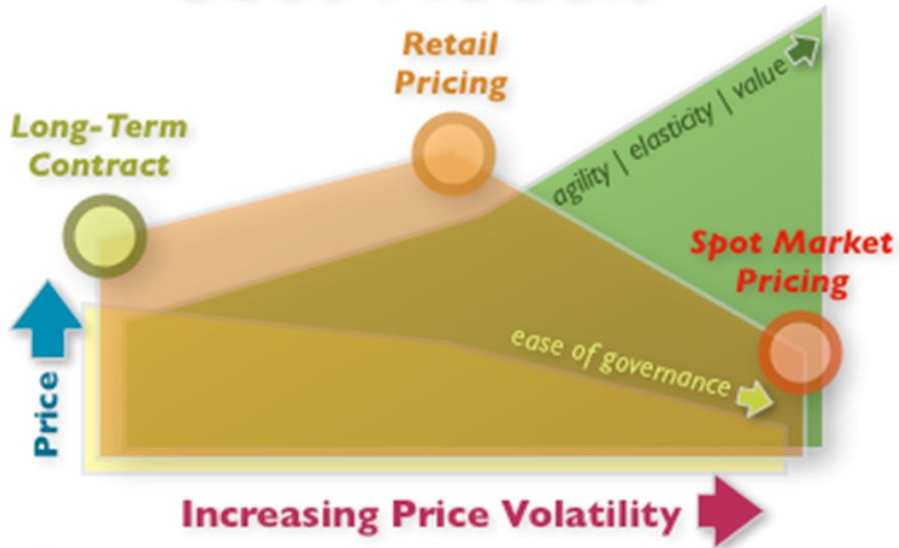
\includegraphics[width=\textwidth]{Figures/intro/cloud_price_models.png}
  \caption{Different Billing Models \cite{cloud_cost_models_figure}}
  \label{fig:DifferentBillingModels}
\end{figure}

The diversity of offerings in the Cloud landscape
leads to practical research questions: how does a service
of a Cloud provider compared to similar offers from other providers? 
How to optimize the process of composite Cloud service selection and
bundling? For example, how does a decision maker compare
the cost/performance features of infrastructure services
offered by AWS, Microsoft Azure, FelxiScale and etc. 
Though branded calculators are available from individual Cloud providers for
calculating service leasing costs, it is not easy for decision
makers to generalize their requirements to fit different
service offers (with various quota and limitations) let alone
computing and comparing costs. A decision
maker may choose one provider for storage intensive
applications and another for computation intensive
applications. 

\subsection{Overwhelming Number of Choices}
\label{subsec:OverwhelmingNumberOfChoices}
It is a cumbersome task for decision makers to manually
read Cloud providers’ documentations for finding out which
services are suitable for building their Cloud-based
application architecture (e.g., a biologist intending to host his
genomics experiment in the Cloud). This problem is further
aggravated due to the rapid emergence of services in the
Cloud landscape.

Burstorm's \cite{Burstorm} survey in 2013 showed that
there were over 426 various compute and
storage service providers with deployments in over 11 072
locations. Even within a particular provider there are different
variations of services. 
For example, Amazon Web Service
(AWS) has 674 different offerings differentiated by price, QoS
features, and locations. In addition to these, every quarter, they add
about four new services, change business models (prices and
terms), and sometimes even add new locations.

\subsection{Evaluating Conflicting Criteria}
\label{subsec:ConflictingRequirements}
The problem is further complicated due to varied service configurations
and application provisioning QoS constraints. 
To be able to select the best mix of service offerings from an abundance of
possibilities, application owners must simultaneously consider
and optimize complex dependence and heterogeneous sets of
criteria (price, features, location, QoS, etc.). 
Often it is not enough to just consider one single type of service.
For example, a content distribution solution not only involves
selecting of an optimal Cloud storage offer, but
company may also need to guarantee the corresponding computing capabilities.
So the desired architecture should be able to both store and processing the data as fast as possible, while minimizing the cost.

The process of matching offers to decision makers’ requirements
involves bundling of multiple related Cloud services,
computing combined cost (under different billing models and
discount offers, considering all possible (or only valuable)
alternatives with selection criteria which can further include: location, minimal memory,
minimal storage capacity, minimal CPU frequency, operating system, etc.

Moreover, as Cloud data centers are distributed across the Internet,
the network QoS (e.g. the data transfer speed and latency) varies. This
variation is dependent on the location of the data center and the
location of the input data stream. This raises
the research question as to how to optimize the process of
choosing the best Compute and Storage services, which are not
only optimized in terms of price, availability, and processing
speed but also offer a good QoS (e.g., the network throughput
and the response delivery latency).

\subsection{Non-trivial Requirements Realization}
\label{subsec:Non-trivialRequirementsRealization}
Current services selection techniques assume user knows their requirements exactly.
For example, assume they know the expected usage of services in the Cloud,
or they have a very rigid budget or QoS expectation. This is not the case, most of the time,
decision makers has a fuzzy picture of what they want to achieve. 
Or users may know their requirements in terms of number of customer requests, server workload,
or some benchmarking metrics, how can we make it easier for users to translate this into appropriate
requirements?
In other situations, they Cloud user may have an existing in-house cluster which they has
some monitoring statistics, how can we incorporated this information when estimating resource usage in the Cloud?

\subsection{Non-standardized User-Unfriendly Interfaces}
\label{subsec:Non-standardizedUser-UnfriendlyInterfaces}
Various system have different user interfaces, some require users to write code for selecting services, for example coding in Structured Query Language (SQL), SPARQL (Protocol and RDF Query Language), Java and so on.
One of the consequences of this is that accessibility to those solutions is limited to decision makers with high IT expertise. 
Similarly when interaction is performed through low-level application programming interfaces (APIs) and command line interfaces. This is inadequate, given the proliferation of Cloud.
This raises a set of research questions: How to develop interfaces that can transform low, system-level programming to easy-to-use drag and drop operations? How do we improve and simplify the process of Cloud service selection and comparison?

\section{Contributions}
\subsection{Cloud Computing Ontology}
\label{sec:CloudComputingOntology}
To address the problem of Ambiguous Terminology and Heterogeneous Service Offers introduced in \Cref{subsec:Non-standardizedAmbiguousTerminology,subsec:HeterogeneousServiceOffers}, we designed the Cloud Computing Ontology (CoCoOn).

CoCoOn defines concepts, features, attributes and relations of Cloud infrastructure services. 
We choose to follow semantic web standards because extensive research
and standardization efforts \cite{DBLP:journals/ao/RomanKLBLSPFBF05,DBLP:conf/www/MartinBMMPSMSS07, DBLP:conf/icws/HallerCMOB05, 5493487, Moscato2011AnAO} have been put into developing
information representation models, with Resource
Description Framework (RDF) \cite{RDF} and Web Ontology Language (OWL) \cite{OWL}. 
In 2012, we proposed the first version of CoCoOn, which models Cloud resources, including
IaaS, SaaS and PaaS; Location and Region; Metric and QoS attributes.
Later on, we extended this model to incorporate popular external vocabularies and adding more annotations.
During which we also revised some of the classes.
CoCoOn facilitates the description of Cloud infrastructure services; 
and through mappings from provider descriptions, facilitates the
discovery of infrastructure services based on their properties and features.

\subsection{Multicriteria Decision Support}
To tackle the problem of Overwhelming Number of Choices and Conflicting Criteria discussed in \Cref{subsec:OverwhelmingNumberOfChoices,subsec:ConflictingRequirements}.
We developed a service selection method adopts an analytic hierarchy process (AHP)-based decision making technique. So optimal selection can be made regardless if the requirements are conflicting or not.
It also enables the handling of multiple quantitative (i.e., numeric) and qualitative (a descriptive and
non-numeric, such as location, CPU architecture, i.e., a 32- or
64-bit operating system) criteria. 
Note that pairwise comparisons \cite{PairwiseComparison} is used to help user determine relative preference among a pool of nonnumerical attributes.
For each pair of criteria, the user is required to provide a subjective
opinion of their relative importance to them.
Then the overall composite weight for each criterion then can be calculated.
Criteria that are taken into consideration during comparison can be grouped into two
categories: the benefit and the cost. “Benefit” groups the “good” criteria
that are meant to be maximized. Similarly, “Cost” groups the “bad” criteria to
be minimized. Based on this, we defined a cost–benefit-ratio-based evaluation function to 
calculate the ranking for Cloud service options.

\subsection{Usage and Cost Estimation}
This thesis further investigates the problem of planning Cloud deployments with non trivial requirements, introduced in \Cref{subsec:Non-trivialRequirementsRealization}.
We suggested a Queuing theory based approach for estimating IaaS usage.
Queuing theory is one of the much studied methods in QoS modelling and control.
From the infrastructure system administrator perspective, we explored ways to apply the Queuing Theory model to estimate the best fit resource allocation for achieving a desired SLA. 
There is a number of studies \cite{lee:10,RodrigoICPP,xuzichuan} which have applied Queuing Theory in their Cloud provisioning mechanism. Since we do not focus on real time provisioning or load balancing, we only use a Queuing Theory based method to estimate the required number of VMs, when other parameters are constrained (i.e. tight budget, performance target on waiting time or throughput).

To calculate Cloud resources' renting costs, the user needs to suggest their planned usage. Our approach has taken into account of different workload patterns during renting cost calculation. For example we defined a number of patterns for users to quickly choose from (i.e. flat/capped usage, regular periodic bursts, liner incremental). 

Alternatively, users may already have some historical
usage statistics, in situations like they want to move in-house systems to the Cloud or from one Cloud/server renting service to another. 
Queuing theory modeling was investigated for usage estimation based on historical customer workload and benchmarking.

\subsection{CloudRecommender}
Finally, the thesis shows how an integrated system, CloudRecommender, can be built from our proposed approaches, for address the problem of Non-standardized User-Unfriendly Interface, introduced in \Cref{subsec:Non-standardizedUser-UnfriendlyInterfaces}.
It allows users to compare and select a Cloud service based on criteria such as the total cost, the maximum size limit for storage and the memory size for compute instance. 
Alternatively users can combines multiple selection criteria by telling the system their preference over interested parameters.
By providing both a web Graphical User Interface (GUI) and an Application Program Interface (API), we exploited the power of a visual programming
language to further enable intuitive Cloud service selection.

QoS Profiler is part of the data collection components.
It collects network QoS statistics from different end points on the Internet to the Cloud data centers.
On top of CloudHarmony's network test service \cite{Cloudharmony_speedtest}, We set up multiple agents at geographically dispersed locations to collect end to end network QoS to various Cloud.
We profiled the network performance continuously, and later used the average for comparison.

\section{Outline of the Thesis}
This thesis provides an in-depth study of the work we have undertaken to address the aforementioned problems in \Cref{sec:research_problem}.
\begin{itemize}
\item \Cref{cha:intro}, which is this chapter, briefly describes the research problems and give an overview of the solutions and the thesis structure.

\item \Cref{cha:background} will give some background information and defining the scope of our work. We will also review related researches in this chapter.

\item \Cref{cha:cocoon} presents the Cloud Computing Ontology we developed for automatically identifying services and representing them in a standard way.

\item \Cref{cha:AHP} presents our decision aid algorithm for ranking Cloud services.

\item \Cref{cha:ResourceUsageEstimation} investigates techniques for planning Cloud deployments with non trivial requirements.

\item \Cref{cha:system} presents our solutions as an integrated system, which we called CloudRecommender.
This section has the implementation details and evaluation of the intelligent decision support framework builds on top of our ontological model and selection and estimation algorithms.
The proposed solution map users’ specified application
requirements to Cloud service configurations, aiding the selection 
of Cloud-based infrastructure services.

\item At last, \Cref{cha:conclusion} summarized our findings and recap the core contributions.
\end{itemize}